
\section{5. Architecture Integration}

\subsection{5.1 Model Support}

\begin{table}[H]
\centering
\begin{tabular}{lllll}
\toprule
\textbf{Architecture} & \textbf{Attention class} & \textbf{RoPE?} & \textbf{GQA?} & \textbf{Verified} \\
\midrule
DistilBERT & `MultiHeadSelfAttention` & No & No &  \\
RoBERTa & `BertSelfAttention` & No & No &  \\
GPT-2 & `GPT2Attention` & No & No &  \\
Qwen3.5 & `Qwen3Attention` & Yes & Yes & {{Q\_VERIFIED}} \\
\bottomrule
\end{tabular}
\end{table}

\subsection{5.2 Weight Transfer}

\subsubsection{5.2.1 DistilBERT (Flat)}

\begin{lstlisting}
q_lin: Linear(768, 768)
k_lin: Linear(768, 768)
v_lin: Linear(768, 768)
out_lin: Linear(768, 768)
\end{lstlisting}

\textbf{Copy:} Direct. \texttt{is\\_nested\\_encoder = False}.

\subsubsection{5.2.2 RoBERTa (Nested)}

\begin{lstlisting}
attention.self.query: Linear(768, 768)
attention.self.key: Linear(768, 768)
attention.self.value: Linear(768, 768)
attention.output.dense: Linear(768, 768)
\end{lstlisting}

\textbf{Copy:} Extract from inner \texttt{self}. \texttt{is\\_nested\\_encoder = True}, skip own 
\texttt{out\\_proj}.

\subsubsection{5.2.3 GPT-2 (Causal)}

\begin{lstlisting}
attn.c_attn: Conv1D(768, 2304)   # fused Q, K, V
attn.c_proj: Conv1D(768, 768)
\end{lstlisting}

\textbf{Copy:} Transpose and split. Direct for \texttt{c\\_proj}.

\subsubsection{5.2.4 Qwen3.5 (GQA + RoPE)}

\begin{lstlisting}
q_proj: Linear(1024, 2048)   # 8 heads $\times$ 256
k_proj: Linear(1024, 512)    # 2 heads $\times$ 256
v_proj: Linear(1024, 512)
o_proj: Linear(2048, 1024)
\end{lstlisting}

\textbf{Copy:} Direct, then \texttt{repeat\\_kv} at runtime. RoPE applied to landmarks 
implicitly via the pooled $Q, K$ (see  5.5).

\subsection{5.3 Injection Algorithm}

\textbf{Algorithm 2:} Inject Primal Attention into a full model
\begin{lstlisting}
Input:  model M, config c, m (landmark count)
Output: M with Primal attention

1:  for   in transformer_layers(M) do
2:      src $\leftarrow$ extract_attention( )
3:      if src is None: continue
4:      new $\leftarrow$ PrimalAttention(config=c, pretrained_attn=src)
5:      replace_attention( , new)
6: end for
\end{lstlisting}

\subsection{5.4 Handling RoPE}

RoPE is applied to $Q, K$ \textbf{before} landmark pooling. This preserves the 
relative positions of the landmark summaries.

\begin{lstlisting}
Q, K = apply_rotary_pos_emb(Q, K, cos, sin, position_ids)
Q_land, K_land = pool_to_landmarks(Q, K, m)
\end{lstlisting}

\subsection{5.5 Handling GQA}

For grouped-query attention, we repeat KV heads \textbf{before} pooling:

\begin{lstlisting}
if num_kv_heads < num_heads:
    K = repeat_kv(K, num_heads // num_kv_heads)
    V = repeat_kv(V, num_heads // num_kv_heads)
\end{lstlisting}

Then landmarks are computed on the repeated KV.

\subsection{5.6 Causality}

For decoder models, causal masking is applied to the \textbf{approximate} attention 
matrix:

\begin{lstlisting}
causal_mask = torch.triu(torch.full((L, L), -1e4), diagonal=1)
attn = attn + causal_mask
\end{lstlisting}

\textbf{Note.} This is not a true causal approximation (landmarks see all tokens), 
but empirically works for generation. See  8.5 for analysis.

\subsection{5.7 Failure Handling}

\texttt{inject\\_primal} returns \texttt{None} on failure and logs the error:

\begin{lstlisting}
try:
    new_attn = PrimalAttention(config=config, pretrained_attn=target, **kwargs)
except Exception:
    raise RuntimeError("copy_weights failed")
\end{lstlisting}

The outer loop can catch this and continue with the next layer.

\subsection{5.8 Parameter Count}

Primal Attention has the \textbf{same parameter count} as MHA:

\begin{table}[H]
\centering
\begin{tabular}{ll}
\toprule
\textbf{Projection} & \textbf{Params} \\
\midrule
$W_Q$ & $d \cdot H d_h$ \\
$W_K$ & $d \cdot H_{kv} d_h$ \\
$W_V$ & $d \cdot H_{kv} d_h$ \\
$W_O$ & $H d_h \cdot d$ \\
\bottomrule
\end{tabular}
\end{table}

With LoRA recovery at rank $r_L$, add $2 r_L (d + d_h H)$ per projection.

\subsection{5.9 Registry}

\begin{lstlisting}
@ATTENTION_REGISTRY.register("primal")
@ATTENTION_REGISTRY.register("primal_attention")
class PrimalAttention(BaseAttention): ...
\end{lstlisting}

\subsection{5.10 Failure Modes}


\begin{figure}[H]
\centering
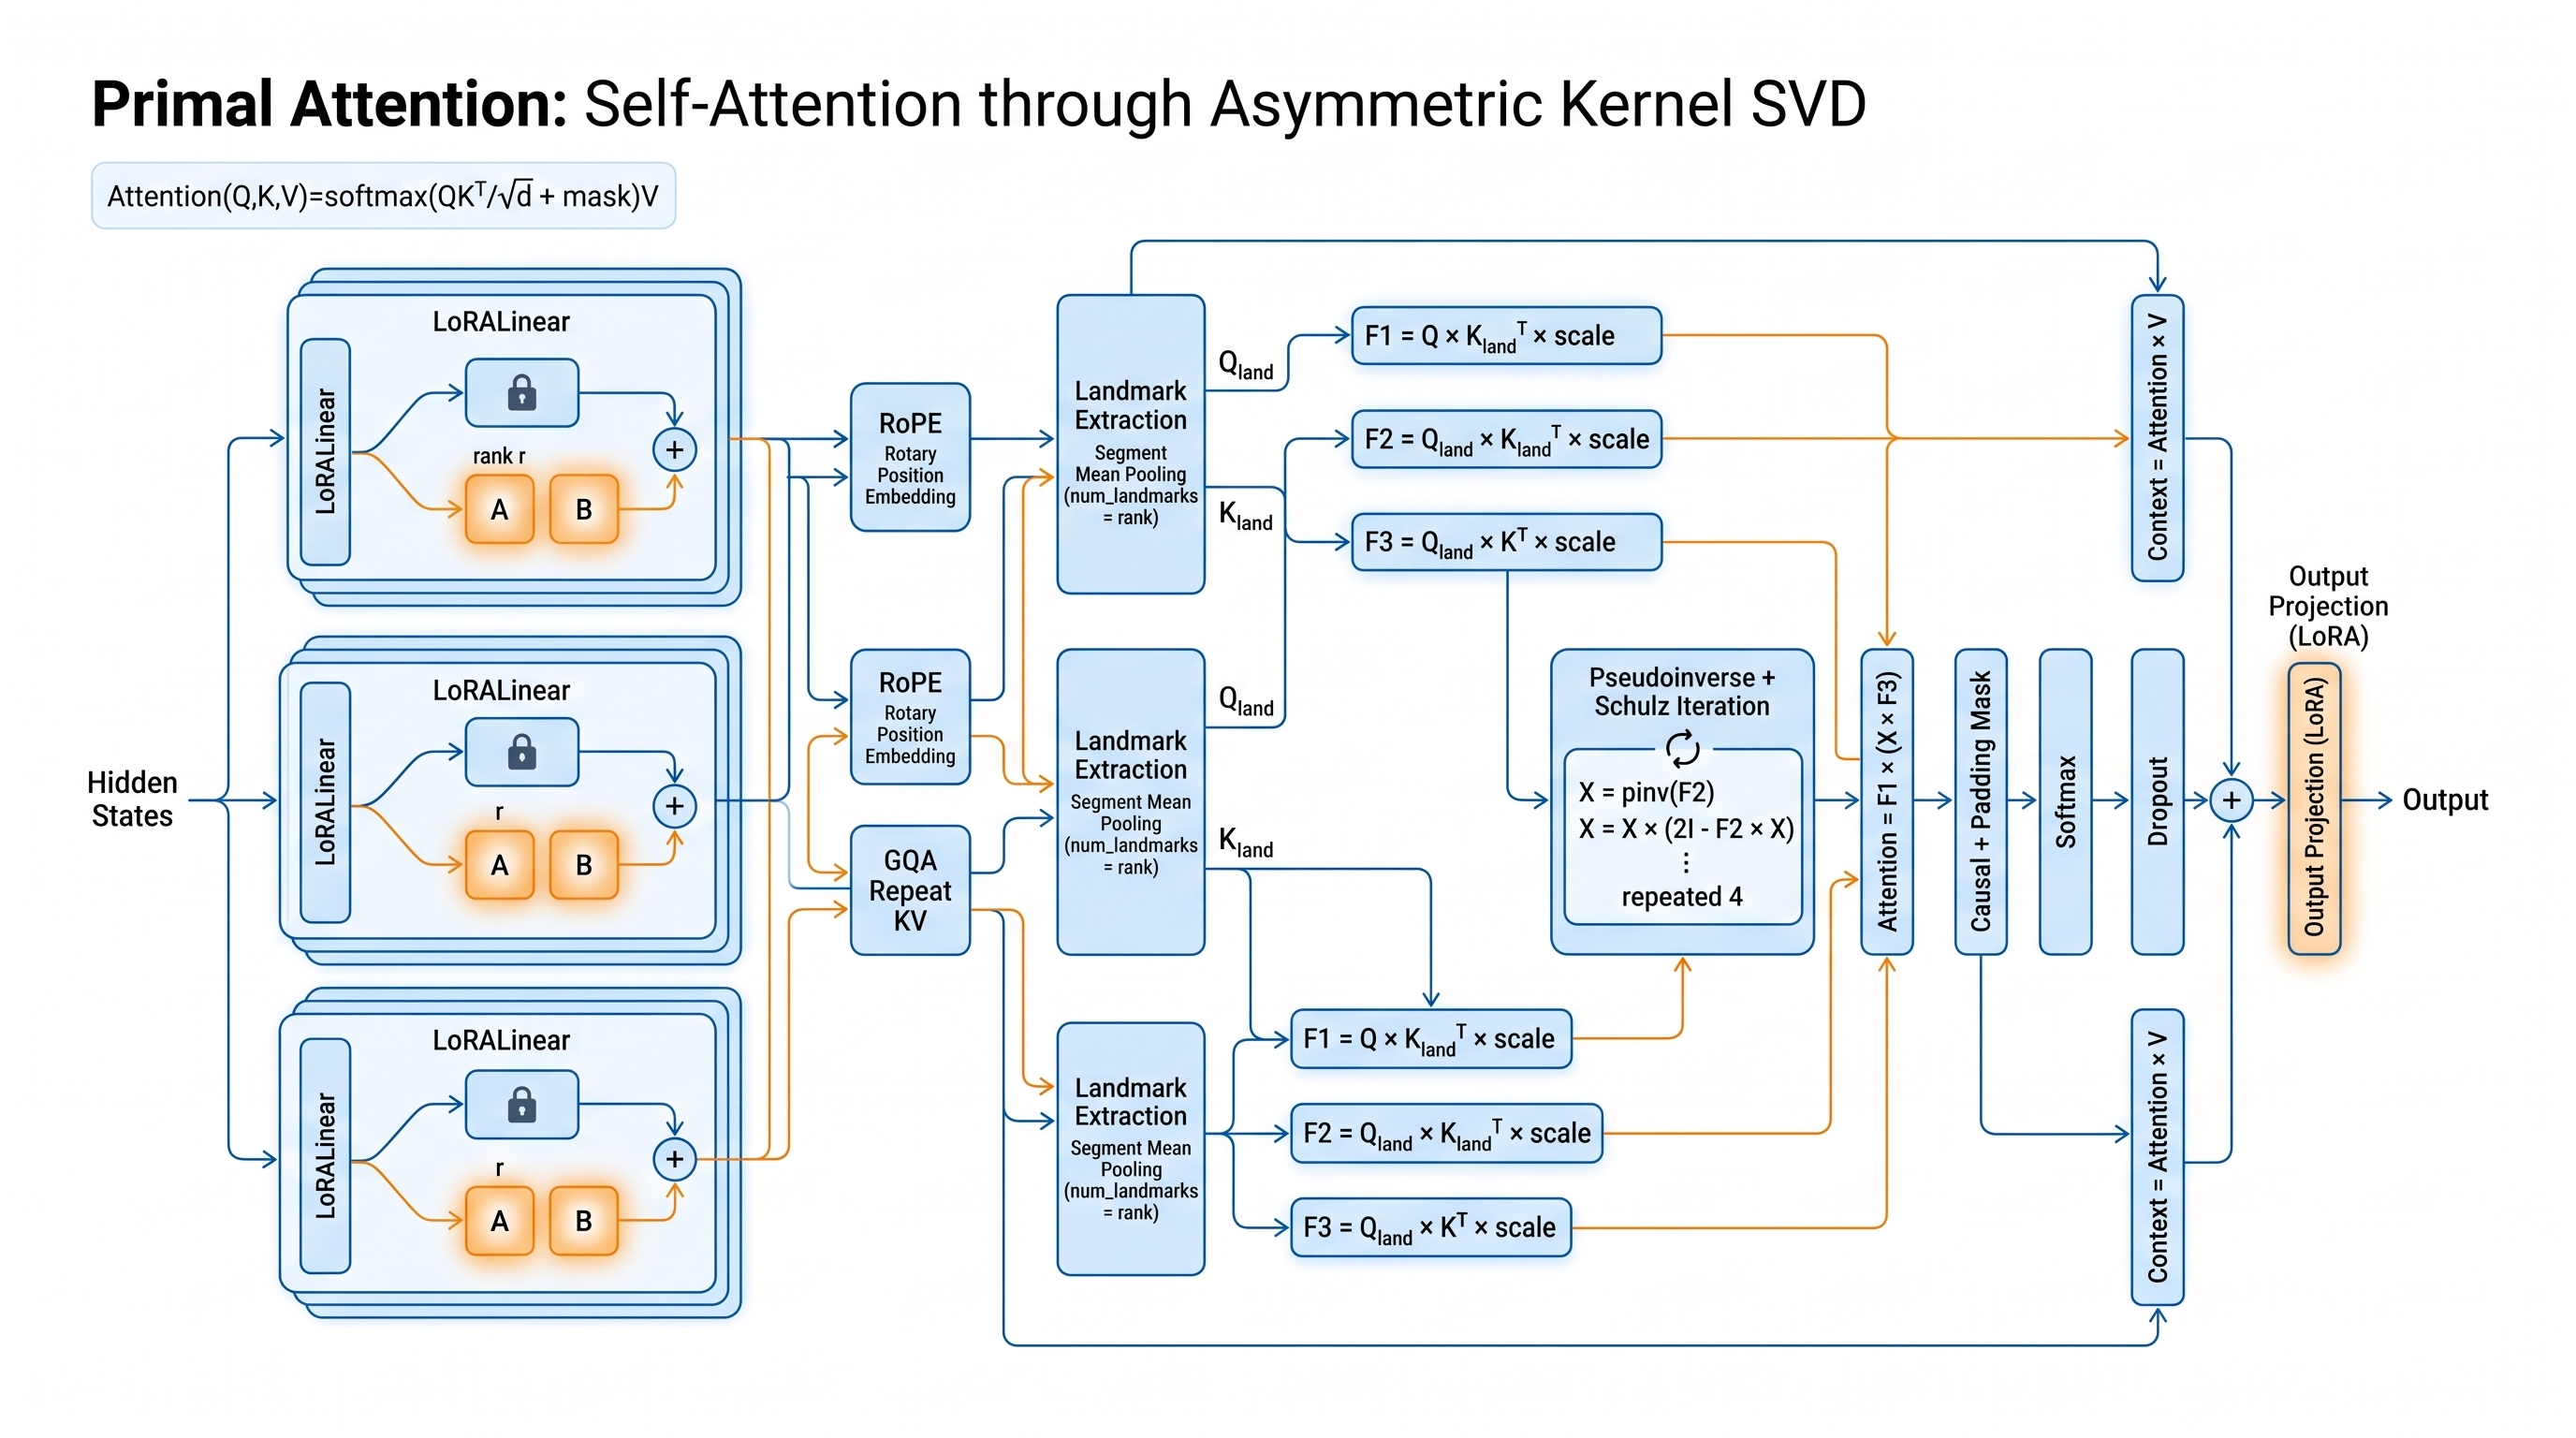
\includegraphics[width=\linewidth]{figures/arch_primal_attention.jpeg}
\caption{Architectural overview of Primal.}
\label{fig:arch_Primal}
\end{figure}
